\chapter{\label{ch:four_level_transduction}Transduction in a Four-Level System in Yb:YVO\textsubscript{4}}

This chapter describes original work on modelling the output power from transduction in a four-level atomic system, which can then be used to calculate transduction efficiency. This builds on concepts used in the three-level transduction models discussed in Chapter \ref{ch:prior_transduction}. Transduction in a four-level system involves multiple atomic transitions that produce output, which may have different phases from each other and therefore interfere. This can affect transduction efficiencies by orders of magnitude, but a three-level model does not account for it. This is applicable to many atomic platforms because the atomic levels used for transduction are almost always part of electronic multiplets, and so a `three-level' transduction system will usually have a fourth level near the optical-separated level. Additionally, this chapter focuses specifically on transduction with atoms coupled directly to waveguides, rather than through cavities as in the prior work, which requires a different formalism to model.

To construct this model, I first constructed a four-level Hamiltonian and resultant Master equation for driven atoms, then used input-output theory to derive an expression for emission from the atoms, and finally expressed the overall emitted power from the entire ensemble as an integral over the inhomogeneous distribution. This thesis also presents numerical methods I developed for implementing the model. After describing this model, this chapter presents a comparison of the output powers computed using the model with those measured in experiments is presented, detailing the process of finding appropriate model parameters.

\section{Target Platform and Benchmark Experimental Data}
\begin{figure}[h!]
\centering
\begin{subfigure}{0.44\textwidth}
    \centering
    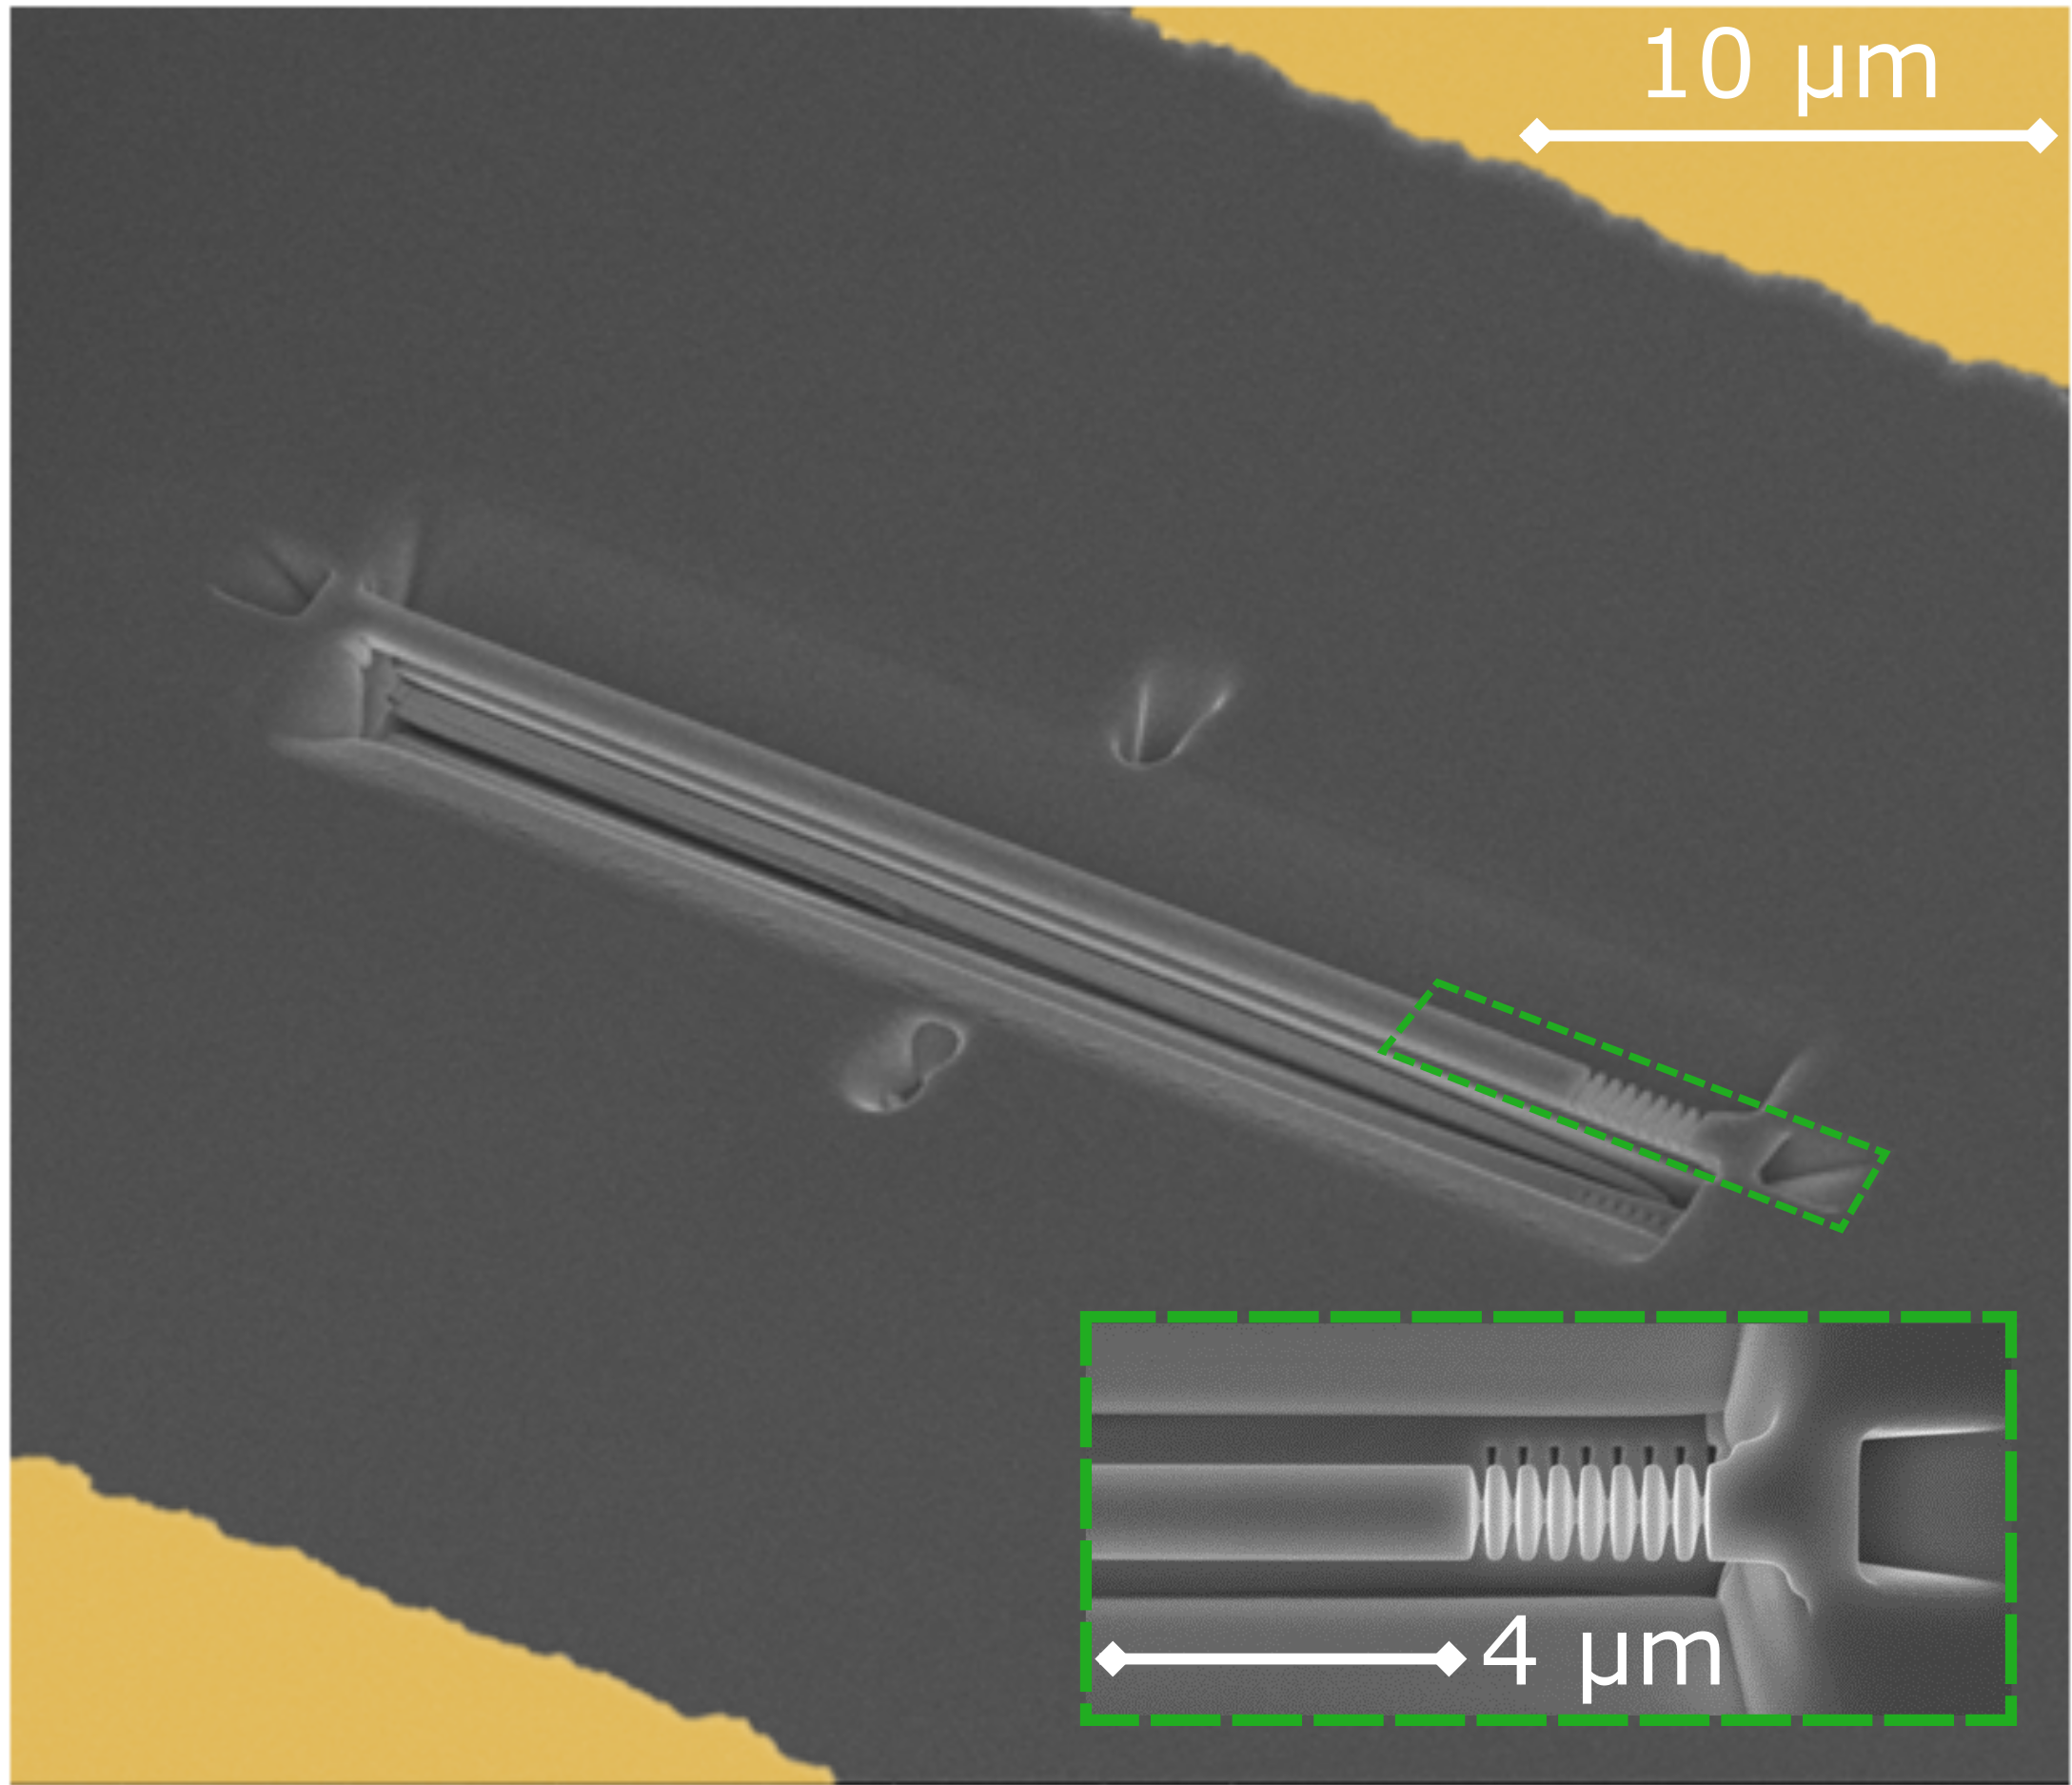
\includegraphics[height=55mm]{4lt-device}
\end{subfigure}
\begin{subfigure}{0.55\textwidth}
    \centering
    \includetikzpicture{four-level-diagram.tikz}
\end{subfigure}
\caption{\label{fig:4lt_device} \textbf{Left} The transduction device in Reference \cite{bartholomew_chip_2020}, consisting of a suspended optical waveguide constructed of \textsuperscript{171}Yb\textsuperscript{3+}:YVO\textsubscript{4}, terminating at a Bragg reflector so that signals enter and exit at the same end. Image credit: Reference \cite{bartholomew_chip_2020}. \textbf{Right} The four-level system in \textsuperscript{171}Yb\textsuperscript{3+}:YVO\textsubscript{4} used, annotated with transition frequencies at $B_z = \qty{2.09}{\milli\tesla}$ and with signal frequencies $\omega_\mu$, $\omega_p$, and $\omega_o$ of the transduction experiments. Shown in grey are the unused levels of the electronic quadruplets.}
\end{figure}

\begin{figure}[h!]
\centering
\includegraphics{4lt-example-scan}
\caption{\label{fig:four_level_transduction_experimental_data} Experimental transduction signals measured by sweeping $\omega_p$ and $\omega_\mu$. Left shows data captured using a weak optical pump in which the transduction signal consists of simple bright spots near the atomic transition frequencies (One for $\omega_p = \omega_{13}$ and one for $\omega_p = \omega_{23}$). Right shows data captured with a strong optical pump, which exhibits nontrivial structure with thin curve-like features. Data credit: Bartholomew et.\ al.\ (unpublished).}
\end{figure}

In constructing a model of four-level transduction. I aim to simulate the experiments described in Bartholomew et.\ al.\ 2020\cite{bartholomew_chip_2020}. This work used an on-chip device (Figure \ref{fig:4lt_device}) consisting of an optical waveguide constructed of \textsuperscript{171}Yb\textsuperscript{3+}:YVO\textsubscript{4} (yttrium orthovanadate doped with ytterbium) crystal, inside a microwave transmission line. For transduction experiments, the device is placed inside a dilution fridge and cooled to $\approx\qty{1}{\kelvin}$.

\textsuperscript{171}Yb\textsuperscript{3+}, the active species in transduction, has a nuclear spin $I=1/2$ and electron spin $S=1/2$. The energy levels of \textsuperscript{171}Yb\textsuperscript{3+} form electronic quadruplets that are non-degenerate (Zeeman-split) in the presence of an external magnetic field. The four levels relevant to the model are the upper two levels of the $^2F_{7/2}$ quadruplet ($\ket{1}$ and $\ket{2}$) and the lower two levels of the $^2F_{5/2}$ quadruplet ($\ket{3}$ and $\ket{4}$), which are separated by microwave transitions within a quadruplet and by near-infrared optical transitions between the quadruplets.

Transduction experiments in Reference \cite{bartholomew_chip_2020} consisted of an optical pump at $\omega_p$ that was swept between and around the $\omega_{13}$ and $\omega_{23}$ transition frequencies and a continuous microwave drive at $\omega_\mu$ that was swept around the $\omega_{34}$ transition frequencies, producing an optical output signal at $\omega_o = \omega_p + \omega_\mu$ through the $\ket{4}\to\ket{1}$ and $\ket{4}\to\ket{2}$ relaxations that is measured and recorded. Examples of these recorded transduction signal strengths are shown in Figure \ref{fig:four_level_transduction_experimental_data}.

This experimental data is used (in Section \ref{sec:4lt_results}) to benchmark the model, specifically a dataset that overlaps with the data published in Reference \cite{bartholomew_chip_2020}, but that also includes some unpublished data\footnote{Given to me by my supervisor who is the lead author of Reference \cite{bartholomew_chip_2020}}. This dataset consists of frequency scans for optical pump powers ranging from $\qty{-40}{\dBm}$ to $\qty{-4}{\dBm}$ inclusive. Published in Reference \cite{bartholomew_chip_2020} are experimental data in a weak optical pump regime in which the transduction signal simply consists of two spots around the two optical transition frequencies, which can be modelled as two separate three-level V-systems that do not significantly interact with each other. However, the unpublished data is in a strong optical pump regime in which the transduction signal contains features that stretch between both optical transitions. Reproducing these features was a goal of my modelling, and this requires a full four-level model.

\section{Driven Atom Hamiltonian}
The effect of the optical pump is represented by Rabi frequencies $\Omega_{13}$ and $\Omega_{23}$ on those respective transitions, because both are driven by the one pump. $\Omega_\mu$ is the Rabi frequency of the microwave drive on the $\ket{3}\to\ket{4}$ transition. Additionally, I include Rabi frequencies $\Omega_{14}$ and $\Omega_{24}$ to represent re-absorption of the emitted light by the atoms, possibly due to some back-reflection or weak cavity-like behaviour in the waveguide. Alternatively, these terms could be used in future modelling work for four-level atoms in cavities. Putting these together using blocks of Equation \ref{eq:two_level_time_dependent_rabi_hamiltonian}, the driven atom Hamiltonian in a static frame is
\begin{equation}
    \hat{H}_\text{static}(\omega'_{12}, \omega'_{13}, \omega'_{14}) =
    \begin{bmatrix}
        0 & 0 & \Omega_{13}^* e^{i\omega_p t} & \Omega_{14}^* e^{i\omega_o t}\\
        0 & \omega'_{12} & \Omega_{23}^* e^{i\omega_p t} & \Omega_{24}^* e^{i\omega_o t}\\
        \Omega_{13} e^{-i\omega_p t} & \Omega_{23} e^{-i\omega_p t} & \omega'_{13} & \Omega_\mu^* e^{i\omega_\mu t}\\
        \Omega_{14} e^{-i\omega_o t} & \Omega_{24} e^{-i\omega_o t} & \Omega_\mu e^{-i\omega_\mu t} & \omega'_{14}
    \end{bmatrix}
\end{equation}
where $\omega'_{ij} = \omega_{ij} - \delta_{ij}$ is, as in Subsection \ref{subs:steady_states}, the $\ket{i}\to\ket{j}$ transition frequency of the atom, which is different for each atom because of inhomogeneous broadening. A unitary transformation to a frame co-rotating with the signals gives a time-independent Hamiltonian
\begin{equation}
    \hat{H}(\delta_{12}, \delta'_p, \delta'_\mu) =
    \begin{bmatrix}
        0 & 0 & \Omega_{13}^* & \Omega_{14}^*\\
        0 & \omega'_{12} & \Omega_{23}^* & \Omega_{24}^*\\
        \Omega_{13} & \Omega_{23} & \delta'_p & \Omega_\mu^*\\
        \Omega_{14} & \Omega_{24} & \Omega_\mu & \delta'_p + \delta'_\mu
    \end{bmatrix}
\end{equation}
which is expressed in terms of detuning variables
\begin{align}
    \delta'_p &= \omega'_{13} - \omega_p = \delta_p - \delta_{13}\\
    \delta'_\mu &= \omega'_{34} - \omega_\mu = \delta_\mu - \delta_{34}.
\end{align}
The Master equation for the atoms is then
\begin{equation}
    \frac{d\hat{\rho}}{dt} =: \mathcal{L}(\delta_{12}, \delta'_p, \delta'_\mu)\hat{\rho} = -i[\hat{H}(\delta_{12}, \delta'_p, \delta'_\mu), \hat{\rho}] + \mathcal{L}_\text{dec}(\delta_{12}, \delta_{34})\hat{\rho}
\end{equation}
where the decoherence operator
\begin{equation}
\begin{split}
    \mathcal{L}_{\text{dec}}\hat{\rho} &= \mathcal{L}_{12}\hat{\rho} + \mathcal{L}_{13}\hat{\rho} + \mathcal{L}_{14}\hat{\rho} + \mathcal{L}_{23}\hat{\rho} + \mathcal{L}_{24}\hat{\rho} + \mathcal{L}_{2d}\hat{\rho} + \mathcal{L}_{3d}\hat{\rho} + \mathcal{L}_{4d}\hat{\rho}\\
    \mathcal{L}_{ij}\hat{\rho} &=
    \begin{cases}
        \begin{split}
            &\frac{\gamma_{ij}(n'_{ij}+1)}{2} \left(2\hat{\sigma}_{ij}\hat{\rho}\hat{\sigma}_{ji} - \hat{\rho}\hat{\sigma}_{jj} - \hat{\sigma}_{jj}\hat{\rho}\right)\\
            &+ \frac{\gamma_{ij}n'_{ij}}{2} \left(2\hat{\sigma}_{ji}\hat{\rho}\hat{\sigma}_{ij} - \hat{\rho}\hat{\sigma}_{ii} - \hat{\sigma}_{ii}\hat{\rho}\right)
        \end{split}
        & \text{$i=1,j=2$ or $i=3,j=4$}\\
        \frac{\gamma_{ij}}{2} \left(2\hat{\sigma}_{ij}\hat{\rho}\hat{\sigma}_{ji} - \hat{\rho}\hat{\sigma}_{j} - \hat{\sigma}_{jj}\hat{\rho}\right) & \text{otherwise}
    \end{cases}\\
    \mathcal{L}_{id}\hat{\rho} &= \frac{\gamma_{id}}{2} \left(2\hat{\sigma}_{ii}\hat{\rho}\hat{\sigma}_{ii} - \hat{\rho}\hat{\sigma}_{ii} - \hat{\sigma}_{ii}\hat{\rho}\right)
\end{split}
\end{equation}
is analogous to that of Equation \ref{eq:three_level_atom_loss_operator}, and depends on the microwave transition shifts via the thermal excitation counts of the microwave transition frequencies $n'_{12}$ and $n'_{34}$. The steady-state density matrix $\hat{\rho}_{SS}(\delta_{12}, \delta'_p, \delta'_\mu)$ can then be found by solving the linear system of the Master equation. In practice, I do this via the real version of the Master equation, as in Equation \ref{eq:real_master_equation}, because an $\mathbb{R}^{4\times 4}$ system of equations is faster to solve than a $\mathbb{C}^{4\times 4}$ system.

\section{Atomic Output}
Adapting from Equation \ref{eq:input_output_theory_output}, the input-output relation for a transition $\ket{i}\leftrightarrow\ket{j}$ of some atom is, up to some phase convention,
\begin{equation}
    \hat{a}_{\text{out},ij} = -\hat{a}_{\text{in},ij} + \sqrt{\gamma_{ij,c}} \hat{\sigma}_{ij}
\end{equation}
where $\gamma_{ij,c} \leq \gamma_{ij}$ is the relaxation rate of the atomic transition through coupling to the waveguide. To form a semiclassical approximation, I replace $\hat{a}_{\text{out},ij} \to \alpha_{\text{out},ij}$, as well as $\hat{a}_{\text{in},ij} \to \alpha_{\text{in},ij} = 0$ because the expectation value of the input is already captured by the Rabi frequencies on the atom Hamiltonian, and $\hat{\sigma}_{ij} \to \rho_{ji,SS}$ where I take the steady state, obtaining
\begin{equation}
    \alpha_{\text{out},ij}(\delta_{12}, \delta'_p, \delta'_\mu) = \sqrt{\gamma_{ij,c}} \rho_{SS,ji}.
\end{equation}
The output power from a given transition, then, is
\begin{equation}
    P_{\text{atom},ij}(\delta_{12}, \delta'_p, \delta'_\mu) = \hbar\omega_o \abs{\alpha_{\text{out},ij}}^2 = \hbar\omega_o \gamma_{ij,c}\abs{\rho_{SS,ji}}^2.
\end{equation}
Recall that there are two transitions producing output in this system, $\ket{1}\leftrightarrow\ket{4}$ and $\ket{2}\leftrightarrow\ket{4}$. The output power from each transition cannot simply be summed to obtain the total atomic output power, because each transition's emission may have different phases, and so they may interfere with each other. Specifically, because this model assumes that the light-matter interactions are through the dipole mechanism, the output has a phase related to that of the matrix element
\begin{equation}
    d_{ij} = \bra{i}\hat{d}_\parallel\ket{j}
\end{equation}
of the component of the dipole moment operator parallel to the emission polarisation. To capture this, I re-express the atomic relaxation rates in terms of complex numbers $C_{ij}$ for which
\begin{align}
    \abs{C_{ij}}^2 &= \gamma_{ij,c} \label{eq:C_ij_magnitude}\\
    \arg C_{ij} &= \arg d_{ij}. \label{eq:C_ij_phase}
\end{align}
Thus, the total atomic output power is
\begin{align}
    P_\text{atom}(\delta_{12}, \delta'_p, \delta'_\mu) &= \hbar\omega_o \abs{C_{14}\rho_{SS,41} + C_{24}\rho_{SS,42}}^2 =: \hbar\omega_o \Gamma_\text{atom}\\
    \Gamma_\text{atom}(\delta_{12}, \delta'_p, \delta'_\mu) &= \abs{C_{14}\rho_{SS,41} + C_{24}\rho_{SS,42}}^2
\end{align}
where $\Gamma_\text{atom}$ is the photon emission rate from the atom.

\section{Ensemble Output}
The total power $P(\delta_p, \delta_\mu)$ from the ensemble can be found as an integral of the single atom power $P_\text{atom}(\delta_{12}, \delta'_p, \delta'_\mu)$ over the inhomogeneous distribution
\begin{align}
    P(\delta_p, \delta_\mu) &= N \iiint p(\delta_{12}, \delta_{13}, \delta_{34}) P_\text{atom}(\delta_{12}, \delta_p-\delta_{13}, \delta_\mu-\delta_{34})\:d\delta_{12}d\delta_{13}d\delta_{34} \label{eq:four_level_total_power_no_approximation}\\
    &= \hbar\omega_oN \iiint p(\delta_{12}, \delta_{13}, \delta_{34}) \Gamma_\text{atom}(\delta_{12}, \delta_p-\delta_{13}, \delta_\mu-\delta_{34})\:d\delta_{12}d\delta_{13}d\delta_{34}
\end{align}
where $p(\delta_{12}, \delta_{13}, \delta_{34})$ is the PDF of the inhomogeneous distribution. I then make the approximation that the inhomogeneous shifts are much smaller than the transition frequencies $\abs{\delta_{ij}} \ll \omega_{ij}$. $\Gamma_\text{atom}$ depends on $\delta_{12}$ only via the shifted transition frequency $\omega'_{12}$, and in this approximation $\omega'_{12} \approx \omega_{12}$, and so $\delta_{12}$ can be ignored. This is not true of the other shifts $\delta_{13}$ and $\delta_{34}$ because $\Gamma_\text{atom}$ depends on them directly. In this approximation, then,
\begin{align}
    P(\delta_p, \delta_\mu) &= \hbar\omega_{o}N \iint p(\delta_{13}, \delta_{34}) \Gamma_\text{atom}(\delta_p-\delta_{13}, \delta_\mu-\delta_{34})\:d\delta_{13}d\delta_{34} \label{eq:four_level_total_power_approximated}\\
    &= \hbar(\omega_{14}-\delta_p-\delta_\mu)N (p * \Gamma_\text{atom}) \label{eq:four_level_total_power_convolution}
\end{align}
where $p(\delta_{13}, \delta_{34}) = \int p(\delta_{12}, \delta_{13}, \delta_{34})\:d\delta_{12}$ is a marginal PDF, and $\omega_o$ has been re-expressed explicitly in terms of the detuning variables. Thus, numerically evaluating a grid of $P(\delta_p, \delta_\mu)$ is a matter of first evaluating a grid of $\Gamma_\text{atom}(\delta'_p, \delta'_\mu)$ and then convolving it with a grid of $p(\delta_{13}, \delta_{34})$, which is much cheaper computationally than evaluating the integral in Equation \ref{eq:four_level_total_power_no_approximation} (or even Equation \ref{eq:four_level_total_power_approximated}) using numerical quadrature because convolutions can be evaluated using Fast Fourier Transform. Furthermore, in the experiments that I am modelling, $\abs{\delta_p}, \abs{\delta_\mu} \ll \omega_{14}$, and so the expression for $\omega_o$ in Equation \ref{eq:four_level_total_power_convolution} simplifies to
\begin{equation}
    P = \hbar\omega_{14}N (p * \Gamma_\text{atom}). \label{eq:four_level_total_power_convolution_approximate}
\end{equation}

\section{Numerical Methods}
As can be seen in Figure \ref{fig:four_level_transduction_experimental_data}, there are thin curve-like features in the transduction signal. When evaluating a grid of $\Gamma_\text{atom}$, these curve features may be subject to grid \textit{aliasing}, in which the relative alignment of the features with the grid points result in unphysical structure in the resulting grid of $\Gamma_\text{atom}$ values, which is then blown up in $P$ by convolution. In this section, I describe the methods I use to implement the model in a manner that is robust to grid aliasing while being computationally cheaper than simply using a finer grid.

\subsection{Grid Aliasing}
A mathematical description of grid aliasing is as follows. Letting $\Delta_{13}$ and $\Delta_{34}$ be the grid spacing of the discretised convolution kernel $p$, the discretised convolution in Equation \ref{eq:four_level_total_power_convolution_approximate} is
\begin{align}
    P(\delta_p, \delta_\mu) &\approx \hbar\omega_{14}N \sum_{(i,j)\in\mathbb{Z}^2} p(i\Delta_{13}, j\Delta_{34}) \Gamma_\text{atom}(\delta_p-i\Delta_{13}, \delta_\mu-j\Delta{34})\\
    &= \iint \underbrace{p(\delta_{13}, \delta_{34}) \Sh_{\Delta_{13}}(\delta_{13}) \Sh_{\Delta_{34}}(\delta_{34})}_\text{convolution kernel} \Gamma_\text{atom}(\delta_p-\delta_{13}, \delta_\mu-\delta_{34})\:d\delta_{13}d\delta_{34}
\end{align}
where $\Sh_T(x)$ is a Dirac comb of period $T$. This means that discretising the convolution in Equation \ref{eq:four_level_total_power_convolution_approximate} is equivalent to discretising the kernel into a weighted Dirac comb. Convolving with this kernel, unlike the original kernel, does not smooth out curve features, but merely displaces them, which is precisely the aliasing mentioned earlier. However, if our grid of $\Gamma_\text{atom}$ contained the integral within the neighbourhood of a grid point instead of just the value at the grid point itself, the discretised convolution would be
\begin{align}
    P(\delta_p, \delta_\mu) &\approx \hbar\omega_{14}N \sum_{(i,j)\in\mathbb{Z}^2} p(i\Delta_{13}, j\Delta_{34}) \int_{i-1/2}^{i+1/2} \int_{j-1/2}^{j+1/2} \Gamma_\text{atom}(\delta_p-i'\Delta_{13}, \delta_\mu-j'\Delta{34})\:di'dj'\\
    &= \iint \underbrace{p([i]\Delta_{13}, [j]\Delta_{34})}_\text{convolution kernel} \Gamma_\text{atom}(\delta_p-i\Delta_{13}, \delta_\mu-j\Delta_{34})\:didj
\end{align}
where $[x]$ is the rounding of $x$ to the nearest integer. This convolution kernel is a step function, which is both closer to the original kernel than a weighted Dirac comb, and smooths out curve features because it is finite everywhere. Evaluating this integral within a neighbourhood for every grid point, however, is equivalent to simply evaluating the discrete convolution with a finer grid, which is the trivial way to deal with aliasing. Instead, my approach is to determine which neighbourhoods contain curve features, and replace only those grid points' values with integrals.

\subsection{Feature Finding}
\begin{figure}[h]
\centering
\includetikzpicture{feature-finding.tikz}
\caption{\label{fig:feature_finding} An illustration of feature finding. The grid squares are neighbourhoods around grid points, and the thick curves represent the features we want to find. The intersections of the feature curves with the neighbourhood edges are shown by circles, and the neighbourhoods containing these features are highlighted grey.}
\end{figure}

To find which neighbourhoods contain curve features, it suffices to simply identify the points of intersection of these features with the edges of neighbourhoods, so that any neighbourhood lying on such an edge contains a curve feature\footnote{Alternatively, curve features could be closed loops contained entirely within that single neighbourhood. I have not observed closed loop features in practice, and even if they do exist, a grid that is coarse enough to contain an entire such loop within a single point's neighbourhood is too coarse to be very useful.}. This is illustrated in Figure \ref{fig:feature_finding}. For an $n\times m$ grid, this process allows all $nm$ neighbourhoods of grid points to be tested for feature presence by testing only the $(n+1)(m+1)$ lines that form edges between them.

As mentioned in Subsection \ref{ssubs:barnett_longdell_numerical_methods}, Reference \cite{barnett_longdell_2020} identified that curve features occur where the discriminant of the characteristic polynomial of the atom Hamiltonian
\begin{equation}
    \Delta(\delta'_p, \delta'_\mu) = \text{Disc}_\lambda\left(\det\left(\hat{H}(\delta'_p, \delta'_\mu)-\lambda\hat{\mathds{1}}\right)\right)
\end{equation}
has its roots. Because the Hamiltonian is Hermitian and therefore its characteristic polynomial has exclusively real roots, this discriminant is uniformly non-negative. This means all roots of the discriminant are `partial' (single-variable) local minima, and it is more numerically stable to identify partial local minima via roots of the discriminant's partial derivative than to directly find roots of the discriminant itself\cite{barnett_msc}. Reference \cite{barnett_longdell_2020} used generic numerical root-finding, but I instead use polynomial-specific root-finding that uses the polynomial coefficients of $\Delta(\delta'_p, \delta'_\mu)$ and its partial derivatives. This has the advantage of finding all roots rather than just one.

\begin{figure}[h!]
\centering
\includegraphics{4lt-pixel-intersections.png}
\caption{\label{fig:pixel_intersections} $\Gamma_\text{atom}$ grids with curve feature intersections identified by along-edge partial local minima (white circles) and across-edge partial local minima (black circles). Left has the same domain as Figure \ref{fig:four_level_transduction_experimental_data} and shows aliasing artefacts along curve features, and right is a close-up around a curve feature, showing duplicate identification and misalignment from the feature's centre.}
\end{figure}

The procedure is as follows.
\begin{enumerate}
    \item Precompute the bivariate polynomial coefficients of $\Delta(\delta'_p, \delta'_\mu)$, $\frac{\partial\Delta}{\partial\delta'_p}(\delta'_p, \delta'_\mu)$, $\frac{\partial^2\Delta}{{\partial\delta'_p}^2}(\delta'_p, \delta'_\mu)$, $\frac{\partial\Delta}{\partial\delta'_\mu}(\delta'_p, \delta'_\mu)$, and $\frac{\partial^2\Delta}{{\partial\delta'_\mu}^2}(\delta'_p, \delta'_\mu)$, because only the detuning variables change over this process.
    \item To find all the intersections along some $\delta'_p$ edge (constant $\delta'_\mu$), evaluate the univariate polynomial coefficients of $\frac{\partial\Delta}{\partial\delta'_p}(\delta'_p)$ for the edge's $\delta'_\mu$, and perform root-finding with them to find all critical points of $\Delta(\delta'_p)$.
    \item Evaluate $\Delta$ at each critical point. Critical points whose values of $\Delta$ are smaller than those of their immediately adjacent critical points are local minima and are therefore taken to be curve feature intersections.
    \item Evaluate the polynomial coefficients of $\frac{\partial\Delta}{\partial\delta'_\mu}(\delta'_p)$ and use them to find critical points of $\Delta(\delta'_\mu)$.
    \item Evaluate the polynomial coefficients of $\frac{\partial^2\Delta}{{\partial\delta'_\mu}^2}(\delta'_p)$ and use them to perform the second derivative test $\frac{\partial^2\Delta}{{\partial\delta'_\mu}^2} \geq 0$ for each critical point of $\Delta(\delta'_\mu)$ to identify local minima.
\end{enumerate}
This process is repeated for each $\delta'_p$ edge, and then vice-versa ($\delta'_p$ and $\delta'_\mu$ swapped) for all $\delta'_\mu$ edges (constant $\delta'_p$).

For each of the two edge directions, both partial local minima along the edge and perpendicular to the edge are identified by this procedure. However, there is an asymmetry between these in that the former use direct comparisons between critical points and the latter use a second derivative test; the latter is to avoid having to evaluate extra $\Delta$ values outside the edge being tested. Furthermore, the second derivative test is done inclusive of exact equality in order to err on the side of false positives rather than false negatives.

\begin{figure}[h!]
\centering
\input{trench-duplication.pgf}
\caption{\label{fig:trench_duplication} Around a curve feature, $\Delta$ often takes the shape of a `trench' which is non-constant at its bottom. When scanning the gradient (arrows) of $\Delta$ in such a region, the gradient flips around on either side, but it is not zero at any point, and so it rotates through the parallel and perpendicular (orange arrows), resulting in this curve feature being found twice.}
\end{figure}

As is shown by Figure \ref{fig:pixel_intersections}, this procedure successfully identifies curve features that produce aliasing artefacts. Additionally, there are curve feature intersections that are found only by the across-edge test, and not the along-edge test, and so this test is necessary to find all grid point neighbourhoods containing curve features. Checking both parallel and perpendicular partial local minima, however, has the side effect of causing many curve features to be identified twice, but this has no effect beyond slightly increasing computational cost. The reasons for this are explained in Figure \ref{fig:trench_duplication}. Additionally, these partial local minima are often very slightly misaligned from the actual curve features, by an amount that is much smaller than most useful grid spacings, and that therefore does not have any significant effect on the final results of this process.

\begin{figure}[h!]
\centering
\includetikzpicture{neighbourhood-integration.tikz}
\caption{\label{fig:neighbourhood_integration} The integration within a single grid point's neighbourhood. The curve feature has an axis-aligned bounding box (dashed) computed from its edge intersections (filled circles) that is wider than it is tall proportional to the neighbourhood's dimensions, and so the outer integral is horizontal and the inner integral (which is represented by the vertical arrows) is vertical. The inner integral's domain is split at curve feature intersections (and surrounding points, which are not shown here).}
\end{figure}

\subsection{Neighbourhood Integration}
Once the points whose neighbourhoods contain curve features are identified, the integral within the neighbourhood must be evaluated using some numerical quadrature scheme. To do this, I use the discriminant once again to perform importance sampling along an inner integral, using Gauss-Lobatto quadrature, as in Reference \cite{barnett_longdell_2020}. For each intersection point, the inner integral's domain is split at intersections with curve features, as well as at addition points surrounding the intersections, with each interval between splits evaluated using a separate instance of Gauss-Lobatto quadrature. If the inner integral is along $\delta'_p$, then for each curve intersection ${\delta'_p}^{(*)}$, the split points are ${\delta'_p}^{(*)}$ itself, ${\delta'_p}^{(*)} \pm \gamma_{ph}$, ${\delta'_p}^{(*)} \pm 3\gamma_{ph}$, and ${\delta'_p}^{(*)} \pm 10\gamma_{ph}$, where $\gamma_{ph} = \gamma_{3d}$ is used as an estimate of the homogeneous linewidth and therefore the thickness of the curve feature. If the inner integral is along $\delta'_\mu$, the splits points from each intersection ${\delta'_\mu}^{(*)}$ are the intersection itself as well as ${\delta'_\mu}^{(*)} \pm \gamma_{\mu h}$, ${\delta'_\mu}^{(*)} \pm 3\gamma_{\mu h}$, and ${\delta'_\mu}^{(*)} \pm 10\gamma_{\mu h}$, where $\gamma_{\mu h} = \gamma_{3d} + \gamma_{4d}$. Split points outside the bounds of the integral (the neighbourhood edges) are excluded.

Reference \cite{barnett_longdell_2020} chose the inner and outer integral axes arbitrarily, but the outer integral would ideally be as close to parallel to the curve feature as possible, because that minimises the distance along the curve between sample points. To handle this, I re-use the curve intersection data computed in the previous step to find an axis-aligned bounding box for the curve feature inside the neighbourhood, and let the outer integral axis be the axis along which this bounding box takes up the largest fraction of the neighbourhood's size (Figure \ref{fig:neighbourhood_integration}).

\section{\label{sec:4lt_parameters}Experimental Parameters for Model}
To summarise, this model requires as input the following parameters:
\begin{itemize}
    \item Microwave transition frequencies $\omega_{12}$ and $\omega_{34}$
    \item Rabi frequencies $\Omega_{13}$, $\Omega_{23}$, $\Omega_{14}$, $\Omega_{24}$, and $\Omega_\mu$
    \item Microwave transition relaxation lifetimes $\tau_{12}$ and $\tau_{34}$ and operating temperature $T$
    \item Optical transition relaxation rates $\gamma_{13}$, $\gamma_{23}$, $\gamma_{14}$, and $\gamma_{24}$
    \item Optical output waveguide couplings $C_{14}$ and $C_{24}$
    \item Inhomogeneous PDF $p(\delta_{13}, \delta_{34})$
    \item Atom count N and optical transition frequency $\omega_{14}$.
\end{itemize}
$N$ merely scales the output signal power uniformly, and therefore does not need much precision, and can be found through trial and error. Reference \cite{bartholomew_chip_2020} quotes an estimate for the operating temperature of $T \approx \qty{1}{\kelvin}$, and a microwave Rabi frequency $\Omega_\mu = 2\pi \times \qty{1}{\mega\hertz}$.

\subsection{Inhomogeneous Broadening}
Reference \cite{bartholomew_chip_2020} specifies the inhomogeneous distribution as Gaussian with standard deviations $\Gamma_{\text{ih},o} \approx \qty{200}{\mega\hertz}$ for optical transitions and $\Gamma_{\text{ih},\mu} \approx \qty{130}{\kilo\hertz}$ for microwave transitions, with a correlation slope of $\num{-120}$ ($\text{optical}/\text{microwave}$) between them. Using the formula
\begin{equation}
    \text{slope} := \frac{\Delta y}{\Delta x} = \frac{\sigma_{xy}}{\sigma_x^2}
\end{equation}
gives a covariance of $\qty{-2.028}{\mega\hertz\squared}$, and so the inhomogeneous PDF is that of the bivariate normal distribution
\begin{align}
    p\left(\vec{\delta} =
    \begin{bmatrix}
        \delta_{13}\\
        \delta_{34}
    \end{bmatrix}\right)
    &=
    \frac{1}{\sqrt{2\pi\det\Sigma}} \exp\left(-\frac{1}{2}\vec{\delta}^T\Sigma^{-1}\vec{\delta}\right)\\
    \Sigma &=
    \begin{bmatrix}
        (\qty{200}{\mega\hertz})^2 & \qty{-2.028}{\mega\hertz\squared}\\
        \qty{-2.028}{\mega\hertz\squared} & (\qty{130}{\kilo\hertz})^2
    \end{bmatrix}.
\end{align}

\subsection{Spin Hamiltonian}
To find the remaining parameters, I make use of the spin Hamiltonians\cite{kindem_characterization_2018} of the two electronic quadruplets in this system
\begin{equation}
    \hat{H}_{g,e} = \mu_B\vec{B}^Tg_{g,e}\vhat{S} + \vhat{I}^TA_{g,e}\vhat{S} \label{eq:spin_hamiltonian_compact}
\end{equation}
where subscripts $g$ and $e$ are indices indicating the ground ($^2F_{7/2}$) and excited ($^2F_{5/2}$) multiplets respectively, $g_{g,e}$ are Zeeman interaction tensors, and $A_{g,e}$ are hyperfine interaction tensors. $\vec{B}$ is the external magnetic field, $\vhat{S} = [\hat{S}_x, \hat{S}_y, \hat{S}_z]^T$ is the electron spin operator and $\vhat{I} = [\hat{I}_x, \hat{I}_y, \hat{I}_z]^T$ is the nuclear spin operator. The symmetry of the crystal site occupied by ytterbium ions\footnote{In the usual crystallography notation, this is the $D_{2d}$ symmetry group} means that the $g_{g,e}$ and $A_{g,e}$ tensors have two eigenvalues, one unique (multiplicity $1$) and one non-unique (multiplicity $2$). Denoting the unique eigenvalues as $g_{\parallel g,e}$ and $A_{\parallel g,e}$ and the non-unique eigenvalues as $g_{\perp g,e}$ and $A_{\perp g,e}$, Equation \ref{eq:spin_hamiltonian_compact} expands into
\begin{equation}
    \hat{H}_{g,e} = \mu_B[g_{\perp g,e}(B_x\hat{S}_x + B_y\hat{S}_y) + g_{\parallel g,e}B_z\hat{S}_z] + A_{\perp g,e}(\hat{I}_x\hat{S_x} + \hat{I}_y\hat{S}_y) + A_{\parallel g,e}\hat{I}_z\hat{S}_z \label{eq:spin_hamiltonian_expanded}
\end{equation}
where it is assumed without generality that $z$ is the unique axis and $x$ and $y$ are the non-unique axes\footnote{In the usual crystallography notation, $c\parallel z$}. The magnetic field in the benchmarking dataset is $\vec{B} = [0, 0, \qty{2.09}{\milli\tesla}]^T$, of which the only nonzero component is $B_z$, but the other components are kept for later calculations regarding magnetic field noise. The interaction tensor elements are shown in Table \ref{tab:spin_hamiltonian_parameters}.

\begin{table}[h]
\centering
\begin{tabular}{c|c}
Parameter & Value\\
\hline
$g_{\perp g}$ & $\num{0.85}$\\
$g_{\parallel g}$ & $\num{-6.08}$\\
$g_{\perp e}$ & $\num{1.7}$\\
$g_{\parallel e}$ & $\num{2.51}$\\
$A_{\perp g}$ & $2\pi \times \qty{675}{\mega\hertz}$\\
$A_{\parallel g}$ & $2\pi \times \qty{-4.82}{\giga\hertz}$\\
$A_{\perp e}$ & $2\pi \times \qty{3.37}{\giga\hertz}$\\
$A_{\parallel e}$ & $2\pi \times \qty{4.86}{\giga\hertz}$\\
\end{tabular}
\caption{\label{tab:spin_hamiltonian_parameters} Interaction tensor elements of the spin Hamiltonian in Equation \ref{eq:spin_hamiltonian_expanded}. $g_{\perp g}$ and $g_{\parallel g}$ are from Reference \cite{ranon_1968}, and the remaining values are from from Reference \cite{kindem_characterization_2018}.}
\end{table}

\subsection{Transition Frequencies}
The eigenvectors of $\hat{H}_g$ are the four levels of the multiplet (Figure \ref{fig:4lt_device}), and so the transition frequencies within a multiplet are simply the difference of the corresponding eigenvalues, which gives us
\begin{align}
    \omega_{12} &= \bra{2}\hat{H}_g\ket{2} - \bra{1}\hat{H}_g\ket{1}\\
    \omega_{34} &= \bra{4}\hat{H}_e\ket{4} - \bra{3}\hat{H}_e\ket{3}
\end{align}
where $\hat{H}_{g,e}$ are evaluated with $B_z = \qty{2.09}{\milli\tesla}$. At zero magnetic field\cite{bartholomew_chip_2020}, $\omega_{13} = 2\pi \times \qty{304501.0}{\giga\hertz}$, and because this is only used to calculate the scale of the output energy (via $\omega_{14} = \omega_{12} + \omega_{23} + \omega_{34}$), this is a good enough approximation of the value at $B_z = \qty{2.09}{\milli\tesla}$.

\subsection{Dephasing Rates}
If we assume that magnetic field noise, which would be caused by the nuclear spin flips in the yttrium and vanadium of the host crystal, is the dominant source of dephasing in this system, then the dephasing rates are proportional to
\begin{equation}
    \gamma_{id} \propto \norm{\frac{d\omega_{1i}}{d\vec{B}}}^2.
\end{equation}
The transition frequency is
\begin{equation}
    \omega_{1i} = \bra{i}\hat{H}_{g,e}\ket{i} - \bra{1}\hat{H}_g\ket{1}
\end{equation}
where the index on the first $\hat{H}_{g,e}$ is $g$ if $i=2$ and $e$ if $i\in\{3,4\}$. Substituting Equation \ref{eq:spin_hamiltonian_expanded} and differentiating, we obtain
\begin{equation}
    \gamma_{id} \propto \norm{g_{g,e} \bra{i}\vhat{S}\ket{i} - g_g \bra{1}\vhat{S}\ket{1}}^2 \label{eq:spin_hamiltonian_dephasing}
\end{equation}
where the index on the first $g_{g,e}$ is the same index as the one on $\hat{H}_{g,e}$. In practice, $\hat{S}_z$ is the only nonzero component of $\vhat{S}$ when restricting these operators to the $(\ket{1}, \ket{2}, \ket{3}, \ket{4})$ basis, and so Equation \ref{eq:spin_hamiltonian_dephasing} becomes
\begin{equation}
    \gamma_{id} \propto \abs{g_{\parallel g,e} \bra{i}\hat{S}_z\ket{i} - g_{\parallel g} \bra{1}\hat{S}_z\ket{1}}^2. \label{eq:spin_hamiltonian_z_dephasing}
\end{equation}

\subsection{Dipole Moments}
The remaining parameters are proportional to dipole moment matrix elements. These include the atomic coupling depolarisation rates
\begin{equation}
    \gamma_{ij,c} \propto \vec{d}_{ij} = \norm{\bra{i}\vhat{d}\ket{j}}^2 \label{eq:depolarisation_proportionality}
\end{equation}
as well as, from Equation \ref{eq:rabi_frequency_dipole_moment},
\begin{equation}
    \Omega_{ij} \propto d_{\parallel ij} \label{eq:rabi_frequency_proportionality}
\end{equation}
where $d_{\parallel ij}$ is the component of $\vec{d}_{ij}$ parallel to the drive polarisation. In this system, both electric and magnetic dipoles are proportional to electron spin
\begin{equation}
    \vhat{d} \propto \vhat{S},
\end{equation}
and so the spin Hamiltonian can once again be used. First of all, Equation \ref{eq:rabi_frequency_proportionality} gives a ratio
\begin{equation}
    \frac{\Omega_{13}}{\Omega_{23}} = \frac{\bra{1}\hat{S}_z\ket{3}}{\bra{2}\hat{S}_z\ket{3}} \label{eq:optical_rabi_frequency_ratio}
\end{equation}
between the optical pump Rabi frequencies, where the fact that $\hat{S}_z$ is the only nonzero spin component has once again been used. The remaining optical Rabi frequencies are set to zero ($\Omega_{14}=0=\Omega_{24}$) because the transduction efficiencies in the benchmarking dataset are quite low ($<10^{-5}$). Second, from Reference \cite{kindem_characterization_2018}, $\gamma_{14}(\vec{B}=\vec{0}) = \qty{1.4}{\kilo\hertz}$ and $\gamma_{23}(\vec{B}=\vec{0}) = \qty{1.3}{\kilo\hertz}$, and optical transitions $\ket{1}\leftrightarrow\ket{3}$ and $\ket{2}\leftrightarrow\ket{4}$ are forbidden at zero magnetic field. In terms of the spin operators, these forbidden transitions are reflected by the fact that
\begin{align}
    \bra{1}\hat{S}_z(\vec{B}=\vec{0})\ket{4} &= -\bra{2}\hat{S}_z(\vec{B}=\vec{0})\ket{3} \neq 0\\
    \bra{1}\hat{S}_z(\vec{B}=\vec{0})\ket{3} &= \bra{2}\hat{S}_z(\vec{B}=\vec{0})\ket{4} = 0.
\end{align}
The fact that dipole-forbidden transitions have depolarisation rates much lower than dipole-permitted transitions shows that these optical depolarisations happen predominantly through dipole emission, and so I set $\gamma_{ij}=\gamma_{ij,c}$. At $B_z=\qty{2.09}{\milli\tesla}$, $\bra{1}\hat{S}_z\ket{3} = \bra{2}\hat{S}_z\ket{4}$ take on a small nonzero value, and $\bra{1}\hat{S}_z\ket{4} = -\bra{2}\hat{S}_z\ket{3}$ decrease in magnitude as the levels hybridise. Using Equation \ref{eq:depolarisation_proportionality},
\begin{equation}
\begin{split}
    \gamma_{14} &= \frac{\abs{\bra{1}\hat{S}_z\ket{4}}^2}{\abs{\bra{1}\hat{S}_z(\vec{B}=\vec{0})\ket{4}}^2} \gamma_{14}(\vec{B}=\vec{0})\\
    \gamma_{23} &= \frac{\abs{\bra{2}\hat{S}_z\ket{3}}^2}{\abs{\bra{2}\hat{S}_z(\vec{B}=\vec{0})\ket{3}}^2} \gamma_{23}(\vec{B}=\vec{0})\\
    \gamma_{13} &= \frac{\abs{\bra{1}\hat{S}_z\ket{3}}^2}{\abs{\bra{2}\hat{S}_z\ket{3}}^2} \gamma_{23}\\
    \gamma_{24} &= \frac{\abs{\bra{2}\hat{S}_z\ket{4}}^2}{\abs{\bra{1}\hat{S}_z\ket{4}}^2} \gamma_{23}\\
\end{split}
\label{eq:optical_relaxation_hybridisation}
\end{equation}
and $C_{14}$ and $C_{24}$ are set accordingly by Equations \ref{eq:C_ij_magnitude} and \ref{eq:C_ij_phase}. From Reference \cite{kindem_control_2020}, $\tau_{12}(\vec{B}=\vec{0}) = \qty{54}{\milli\second}$, and so
\begin{equation}
    \tau_{12} = \frac{\abs{\bra{1}\hat{S}_z(\vec{B}=\vec{0})\ket{2}}^2}{\abs{\bra{1}\hat{S}_z\ket{2}}^2} \tau_{12}(\vec{B}=\vec{0}). \label{eq:tau_12_hybridisation}
\end{equation}
In the absence of data on $\tau_{34}$, I set it to $\qty{10}{\milli\second}$, to match the order of magnitude of $\tau_{12}$.

\subsection{Optical Pump Calibration}
From Equation \ref{eq:rabi_frequency_dipole_moment}, $\Omega_{23} \propto \sqrt{P}$ where $P$ is the pump power. The equation for this proportionality, appropriately calibrated, is
\begin{equation}
    \Omega_{23} = \frac{\Omega_{23,\text{ref}}\sqrt{\eta}}{\sqrt{P_\text{ref}}} \sqrt{P}
\end{equation}
where $(\Omega_{23,\text{ref}}, P_\text{ref})$ is some known `reference' Rabi frequency-power pair for calibration, and $\eta$ is the efficiency with which power from the source makes it into the waveguide. Reference \cite{bartholomew_chip_2020} contains a frequency-power pair $(\Omega_{23,\text{ref}}=2\pi\times\qty{6}{\mega\hertz}, P_\text{ref}=\qty{2}{\micro\watt})$, and my supervisor provided data with which to calibrate the efficiency to $\eta=\num{0.055}$ (Appendix \ref{ap:4lt_power_calibration}). 

\section{\label{sec:4lt_results}Results}
\begin{figure}[h]
\centering
\includegraphics{4lt-model-scan}
\caption{\label{fig:4lt_model_scan} Power-frequency grids from the model when obeying the constraints found in Section \ref{sec:4lt_parameters} (left) and when disobeying those constraints (middle) as compared with the experimental data (right) shown in Figure \ref{fig:four_level_transduction_experimental_data}, with optical pump power $\qty{-4}{\dBm}$. All three plots have the same frequency and colour scales. A simple noise model is used in this comparison.}
\end{figure}

To evaluate the model, I computed power-frequency grids with frequency domain and input parameters corresponding to the experimental data. Because the model does not include the noise in the experimental apparatus, I add simulated noise to the computed power. This consists of random samples from the experimental frequency sweep with $\qty{-40}{\dBm}$ optical pump power, which contains no discernible transduction signal, only noise. A comparison of the resultant power-frequency grids with experimental data is shown in Figure \ref{fig:4lt_model_scan}.

After the analysis in Section \ref{sec:4lt_parameters}, the remaining free parameters are $N$ and $\gamma_{2d}$, as well as some leeway in adjusting $\Omega_{23}$ since the calibration parameters $\Omega_{23,\text{ref}}$ and $P_\text{ref}$ have only one significant figure of precision. I adjusted these free parameters to find a set of parameters that best replicated the experimental data, which resulted in $N=\num{1e14}$, $\gamma_{2d}=\qty{10}{\kilo\hertz}$, and an adjustment to the $\Omega_{23}$ calibration of $P_\text{ref}=\qty{1.7}{\micro\watt}$.

This showed only superficial qualitative agreement, and so I next adjusted the parameters while breaking the constraints identified in Section \ref{sec:4lt_parameters}, finding better agreement with $N=\num{1e10}$, $\tau_{12}(\vec{B}=\vec{0})=\qty{1}{\micro\second}$, and a modified \textit{optical hybridisation ratio}
\begin{equation}
    \frac{\abs{\bra{1}\hat{S}_z\ket{3}}}{\abs{\bra{2}\hat{S}_z\ket{3}}} = \frac{\abs{\bra{2}\hat{S}_z\ket{4}}}{\abs{\bra{1}\hat{S}_z\ket{4}}} \approx \num{0.12} \to \num{0.38},
\end{equation}
and all downstream variables $\tau_{12}$, $\gamma_{13}$, $\gamma_{23}$, $\gamma_{14}$, $\gamma_{24}$, and $\Omega_{13}$ modified accordingly using Equations \ref{eq:tau_12_hybridisation}, \ref{eq:optical_relaxation_hybridisation}, and \ref{eq:optical_rabi_frequency_ratio}, preserving the phase of $\Omega_{13}/\Omega_{23}$.

In both model grids, we see dark curve features, corresponding to destructive interference between the two output transitions, that span the distance between the two atomic transition frequencies $\omega_{23}$ and $\omega_{13}$, which are also seen in the experimental data, and can only be produced by a model that accounts for all four levels and both output transitions simultaneously. However, their locations are much more accurate to the experimental data in the model grid evaluated using the constraint-breaking parameter set. Furthermore, the constraint-obeying grid has a dynamic range much greater than that of the experimental data, with the bright transduction signal oversaturating the colour scale (or else, by a downscaling of $N$, losing the dark features in the noise.), while the constraint-breaking grid gives much better quantitative agreement.

However, even the better of the two grids is not perfect. The main discrepancy is that the bright transduction signals are much broader than in the experimental data. Additionally, the region immediately surrounding $(\omega_\mu, \omega_p) = (\omega_{34}, \omega_{13})$ is darker than its surroundings in the model grid, whereas the opposite is true in the experimental data. What is not problematic, however, is that the features in model grid are translated along the $\delta_{\mu}$ axis (horizontal in the plot) compared to their locations in the experimental data; this shift is by an amount smaller than the uncertainty\footnote{Implied by the number of significant figures} on $A_{\perp e} = \omega_{34}(\vec{B}=\vec{0}) = 2\pi \times \qty{3.37}{\giga\hertz}$ of $\pm 2\pi\times\qty{5}{\mega\hertz}$. Indeed, this model and experimental data could be used, in theory, to find a more precise estimate of that spin Hamiltonian parameter.

Given that the experimental parameters relevant to the model are not known with certainty, especially since parameters ostensibly constrained by theory must be modified to obtain good agreement with experiment, these discrepancies between model and experiment do not necessarily indicate deficiencies in the model. Instead, they might simply be the result of input parameters to the model not matching those used in the experiments that produced the benchmarking data.

\subsection{Accounting for Constraint Breaking}
In this subsection, I offer some possible explanations for why the true parameters of the benchmark experiment might be the constraint-breaking parameters that give good model-experiment agreement, and why they might be different to those calculated in Section \ref{sec:4lt_parameters}.

\subsubsection{Lifetime $\tau_{12}$}
The depolarisation lifetime of a dipole transition depends not only on the dipole moment matrix element of the transition, which is a fundamental constant of the emitter, but also on the per-photon electromagnetic field strength, which depends on the environment surrounding the emitter, i.e.\ whether it is in free space, a waveguide, or a resonator, and the specific geometries of the latter two. Equivalently, and more commonly, this is expressed in terms of the local density of states (LDOS) around the emitter.

Reference \cite{kindem_control_2020}, which measured $\tau_{12}(\vec{B}=\vec{0})$, did so in a device different to that with which the experimental data was produced, and so this could potentially be source of this discrepancy.

\subsubsection{Hybridisation Ratio}
\begin{figure}[h]
\centering
\includegraphics{4lt-scan-hyperbolas}
\caption{\label{fig:4lt_scan_hyperbolas} Manual axis-aligned hyperbola fits to the dark features surrounding the $\omega_{13}$ and $\omega_{23} $transitions. The (red) hyperbola surrounding the $\omega_{23}$ (lower) transition has a centre of $(3369.2, 652)$ in the axis coordinates shown and a vertex-to-vertex distance of $2\pi \times \qty{66}{\mega\hertz}$. The (black) hyperbola surrounding the $\omega_{13}$ (upper) transition has a centre of $(3370.1, 1350)$ and a vertex-to-vertex distance of $2\pi \times \qty{12.6}{\mega\hertz}$. The ratio of these vertex-to-vertex distances is $\num{0.19}$.}
\end{figure}

\noindent The hybridisation ratio of $\num{0.38}$ was identified using the experimental data. Specifically, the hyperbolic dark features\footnote{\textit{Rabi splittings}} surrounding the transition frequencies are expected from theory to have vertex-to-vertex distances proportional to the Rabi frequencies on the transitions\cite{baur_2009}. Measuring these (Figure \ref{fig:4lt_scan_hyperbolas}) yielded a ratio of $\num{0.19}$. This does not produce a good fit in the model, but its double, $\num{0.38}$, does; it is unclear why this factor of two is needed.

This leaves the question of why the hybridisation ratio is so large, compared to the value at $B_z=\qty{2.09}{\milli\tesla}$ of $\num{0.12}$. One possibility would be that that magnetic field value is wrong, and the magnetic field is in fact much stronger than that. As Figure \ref{fig:4lt_hybridisation_ratio} shows, a value of $B_z\approx\qty{8}{\milli\tesla}$ would produce a hybridisation ratio of $\num{0.38}$. However, such a strong magnetic field would create Zeeman shifts much larger than those observed in the experimental data, translating every feature by a substantial amount. Therefore, such a magnetic field strength is implausible.

\begin{figure}[h]
\centering
\includegraphics{4lt-hybridisation-ratio}
\caption{\label{fig:4lt_hybridisation_ratio} A plot of hybridisation ratio vs magnetic field strength $B_z$. $B_z=\qty{2.09}{\milli\tesla}$ (dashed vertical line) and hybridisation ratio $\norm{\vec{d}_{13}}^2/\norm{\vec{d}_{23}}^2 = \num{0.38}$ (dotted horizontal line) are superimposed, with the latter intersecting the curve at about $B_z\approx\qty{8}{\milli\tesla}$.}
\end{figure}
